\documentclass{article}
\usepackage[utf8]{inputenc}
\usepackage[T1]{fontenc}
\usepackage{booktabs}
\usepackage{graphicx}
\usepackage{geometry}
\usepackage{amsmath}
\geometry{margin=1in}

\title{Redundant Experiments: Independent Re-Run Comparison}
\author{}
\date{}

\begin{document}
\maketitle

\noindent This document compares the results in \texttt{paper.tex} (run by Diego) against
an independent re-run of the same eval sweep (results supplied by Riyasat, unpacked under
\texttt{evals/riyasat/}), using the exact same plots and table layout as the main paper for
direct comparison. \textbf{Caveat:} Riyasat's export did not include OLMoE's
\emph{Working-set reward}, \emph{Option-critic controller}, or \emph{MELINOE} runs -- those
three rows below are copied in from Diego's own results (not an independent re-run) purely
to keep the table complete; do not read them as a redundancy check. Every other row/figure
here \emph{is} an independent re-run and should be compared against the corresponding
number in \texttt{paper.tex}.

\section{Downstream Task and Working-Set Metrics}

\begin{table}[h]
\centering
\small
\caption{Phi-tiny-MoE-instruct, redundant run (1024 held-out prompts, $c=4$, top-2). Base
row is absolute; other rows are $\Delta$ from this run's own base model. Compare against
Table~1 of \texttt{paper.tex}.}
\resizebox{\textwidth}{!}{%
\begin{tabular}{l ccccc | ccc}
\toprule
 & \multicolumn{5}{c|}{lm-eval-harness score ($\Delta$ from base)} & \multicolumn{3}{c}{working-set efficiency} \\
Objective & MMLU & MMMLU & GSM8K & HumanEval & MATH & Hit ratio & Misses & ECI \\
\midrule
Base (untuned)          & 0.619 & 0.344 & 0.624 & 0.031 & 0.085 & 0.570 & 648.6 & 0.891 \\
\midrule
Causal LM alone (SFT)   & +0.003 & $-$0.018 & +0.017 & 0.000  & $-$0.006 & 0.568 & 789.3 & 0.892 \\
Working-set reward       & $-$0.023 & +0.011 & $-$0.055 & +0.012 & $-$0.011 & 0.621 & 437.6 & 0.888 \\
Working-set reward + SFT & $-$0.004 & +0.006 & $-$0.002 & $-$0.006 & $-$0.006 & \textbf{0.789} & \textbf{401.6} & 0.691 \\
Option-critic controller & $-$0.024 & $-$0.020 & $-$0.110 & $-$0.012 & $-$0.076 & \textbf{1.000} & \textbf{0.1} & 0.279 \\
MELINOE                 & 0.000  & $-$0.010 & $-$0.138 & $-$0.019 & $-$0.069 & 0.879 & 239.0 & 0.674 \\
\bottomrule
\end{tabular}%
}
\end{table}

\begin{table}[h]
\centering
\small
\caption{OLMoE-1B-7B, redundant run where available (1024 held-out prompts, $c=16$,
top-8). Base and SFT rows are an independent re-run; the last three rows are carried over
from \texttt{paper.tex} (see caveat above). Compare against Table~2 of \texttt{paper.tex}.}
\resizebox{\textwidth}{!}{%
\begin{tabular}{l ccccc | ccc}
\toprule
 & \multicolumn{5}{c|}{lm-eval-harness score ($\Delta$ from base)} & \multicolumn{3}{c}{working-set efficiency} \\
Objective & MMLU & MMMLU & GSM8K & HumanEval & MATH & Hit ratio & Misses & ECI \\
\midrule
Base (untuned)          & 0.565 & 0.377 & 0.680 & 0.311 & 0.056 & 0.686 & 1879.5 & 0.895 \\
\midrule
Causal LM alone (SFT)   & $-$0.021 & $-$0.014 & $-$0.095 & $-$0.201 & $-$0.012 & 0.678 & 1957.9 & 0.897 \\
\midrule
\multicolumn{9}{l}{\emph{-- rows below are carried over from Diego's run, not an independent re-run --}} \\
\midrule
Working-set reward       & $-$0.001 & $-$0.010 & $-$0.007 & +0.018 & +0.004 & 0.759 & 1004.2 & 0.895 \\
Option-critic controller & $-$0.038 & $-$0.066 & $-$0.138 & $-$0.171 & $-$0.054 & 0.684 & 2012.7 & 0.888 \\
MELINOE                 & $-$0.073 & $-$0.055 & $-$0.245 & $-$0.232 & $-$0.054 & 0.763 & 1541.9 & 0.838 \\
\bottomrule
\end{tabular}%
}
\end{table}

\section{Downstream Accuracy vs. Working-Set Locality}

\begin{figure}[h]
\centering
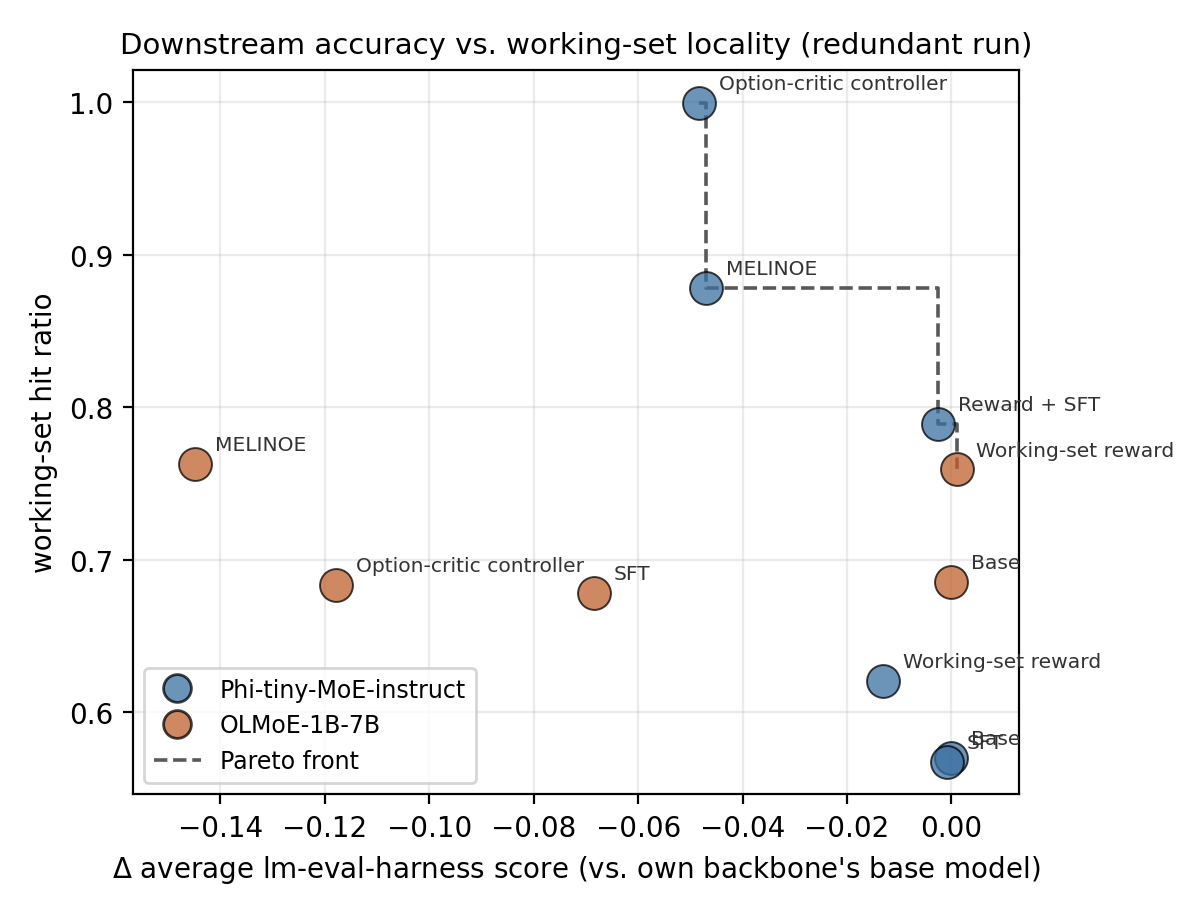
\includegraphics[width=0.75\textwidth]{figures_redundant/delta_score_vs_hit_ratio_redundant.png}
\caption{Redundant run's version of Figure~1 in \texttt{paper.tex}: change in average
lm-eval-harness score versus working-set hit ratio, relative to each backbone's own base
model in \emph{this} run. Compare the shape of the Pareto front and the relative position
of each labeled point against the main paper's figure.}
\end{figure}

\section{Prompt-Conditioned Capacity Sweep}

Riyasat's export included the full prompt-conditioned cache-size sweep for \emph{both}
backbones (Phi-tiny-MoE at $c\in\{2,4,8\}$ and OLMoE at $c\in\{8,16,32\}$), unlike the main
paper which only had OLMoE's sweep available at submission time. The two capacity ranges
are put on a common x-axis as \% of each backbone's total expert count, so both curves can
be read on one plot (Phi: 16 experts, OLMoE: 64 experts -- $c=2,4,8$ and $c=8,16,32$ land on
the same 12.5\%/25\%/50\% marks).

\begin{table}[h]
\centering
\small
\caption{Prompt-conditioned policy, redundant run, swept over capacity.}
\begin{tabular}{lccc}
\toprule
Backbone & Capacity $c$ & Hit ratio & Tokens/s (base-normalized) \\
\midrule
Phi-tiny-MoE-instruct & 2  & 0.651 & 181.0 \\
Phi-tiny-MoE-instruct & 4  & 0.831 & 184.4 \\
Phi-tiny-MoE-instruct & 8  & \textbf{0.944} & \textbf{186.3} \\
\midrule
OLMoE-1B-7B & 8  & 0.508 & 259.4 \\
OLMoE-1B-7B & 16 & 0.741 & 272.3 \\
OLMoE-1B-7B & 32 & \textbf{0.903} & \textbf{279.5} \\
\bottomrule
\end{tabular}
\end{table}

\begin{figure}[h]
\centering
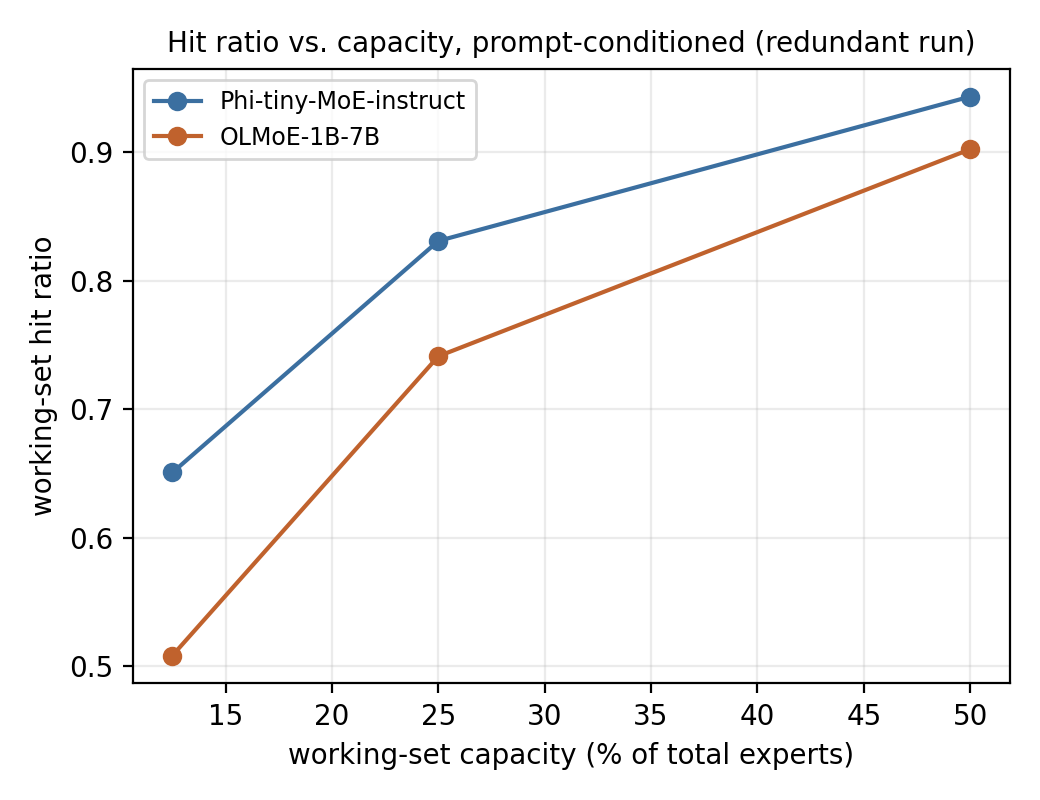
\includegraphics[width=0.48\textwidth]{figures_redundant/scaling_hit_ratio_redundant.png}
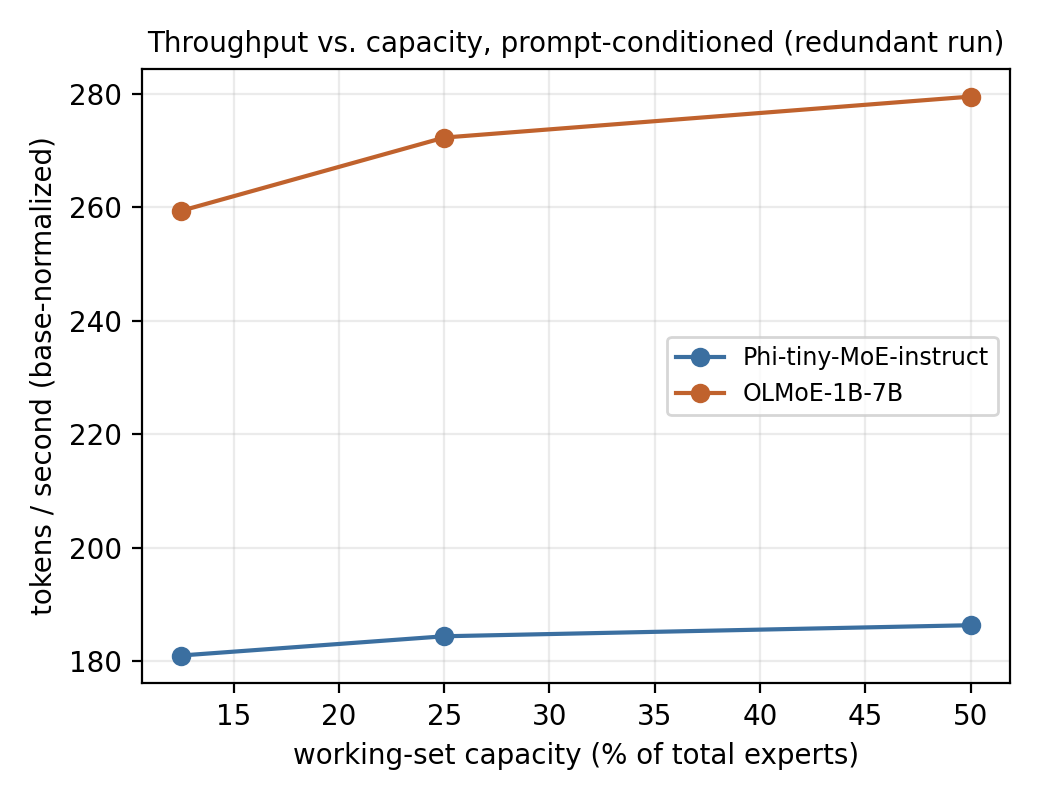
\includegraphics[width=0.48\textwidth]{figures_redundant/scaling_tokens_per_second_redundant.png}
\caption{Prompt-conditioned hit ratio (left) and base-normalized tokens/second (right) vs.
working-set capacity, as a fraction of each backbone's total expert count, for the
redundant run. Compare against \texttt{paper.tex}'s OLMoE-only scaling figures (Appendix
figures for the main paper) -- this version additionally has the Phi-tiny-MoE curve, not
available from Diego's own sweep at submission time.}
\end{figure}

\section{Expert Routing Traces (Redundant Run)}

Routing traces for the objectives that were independently re-run. OLMoE's working-set
reward, option-critic controller, and MELINOE traces are omitted here since those rows are
carried over from Diego's run (identical by construction, not a useful comparison point).

\begin{figure}[h]
\centering
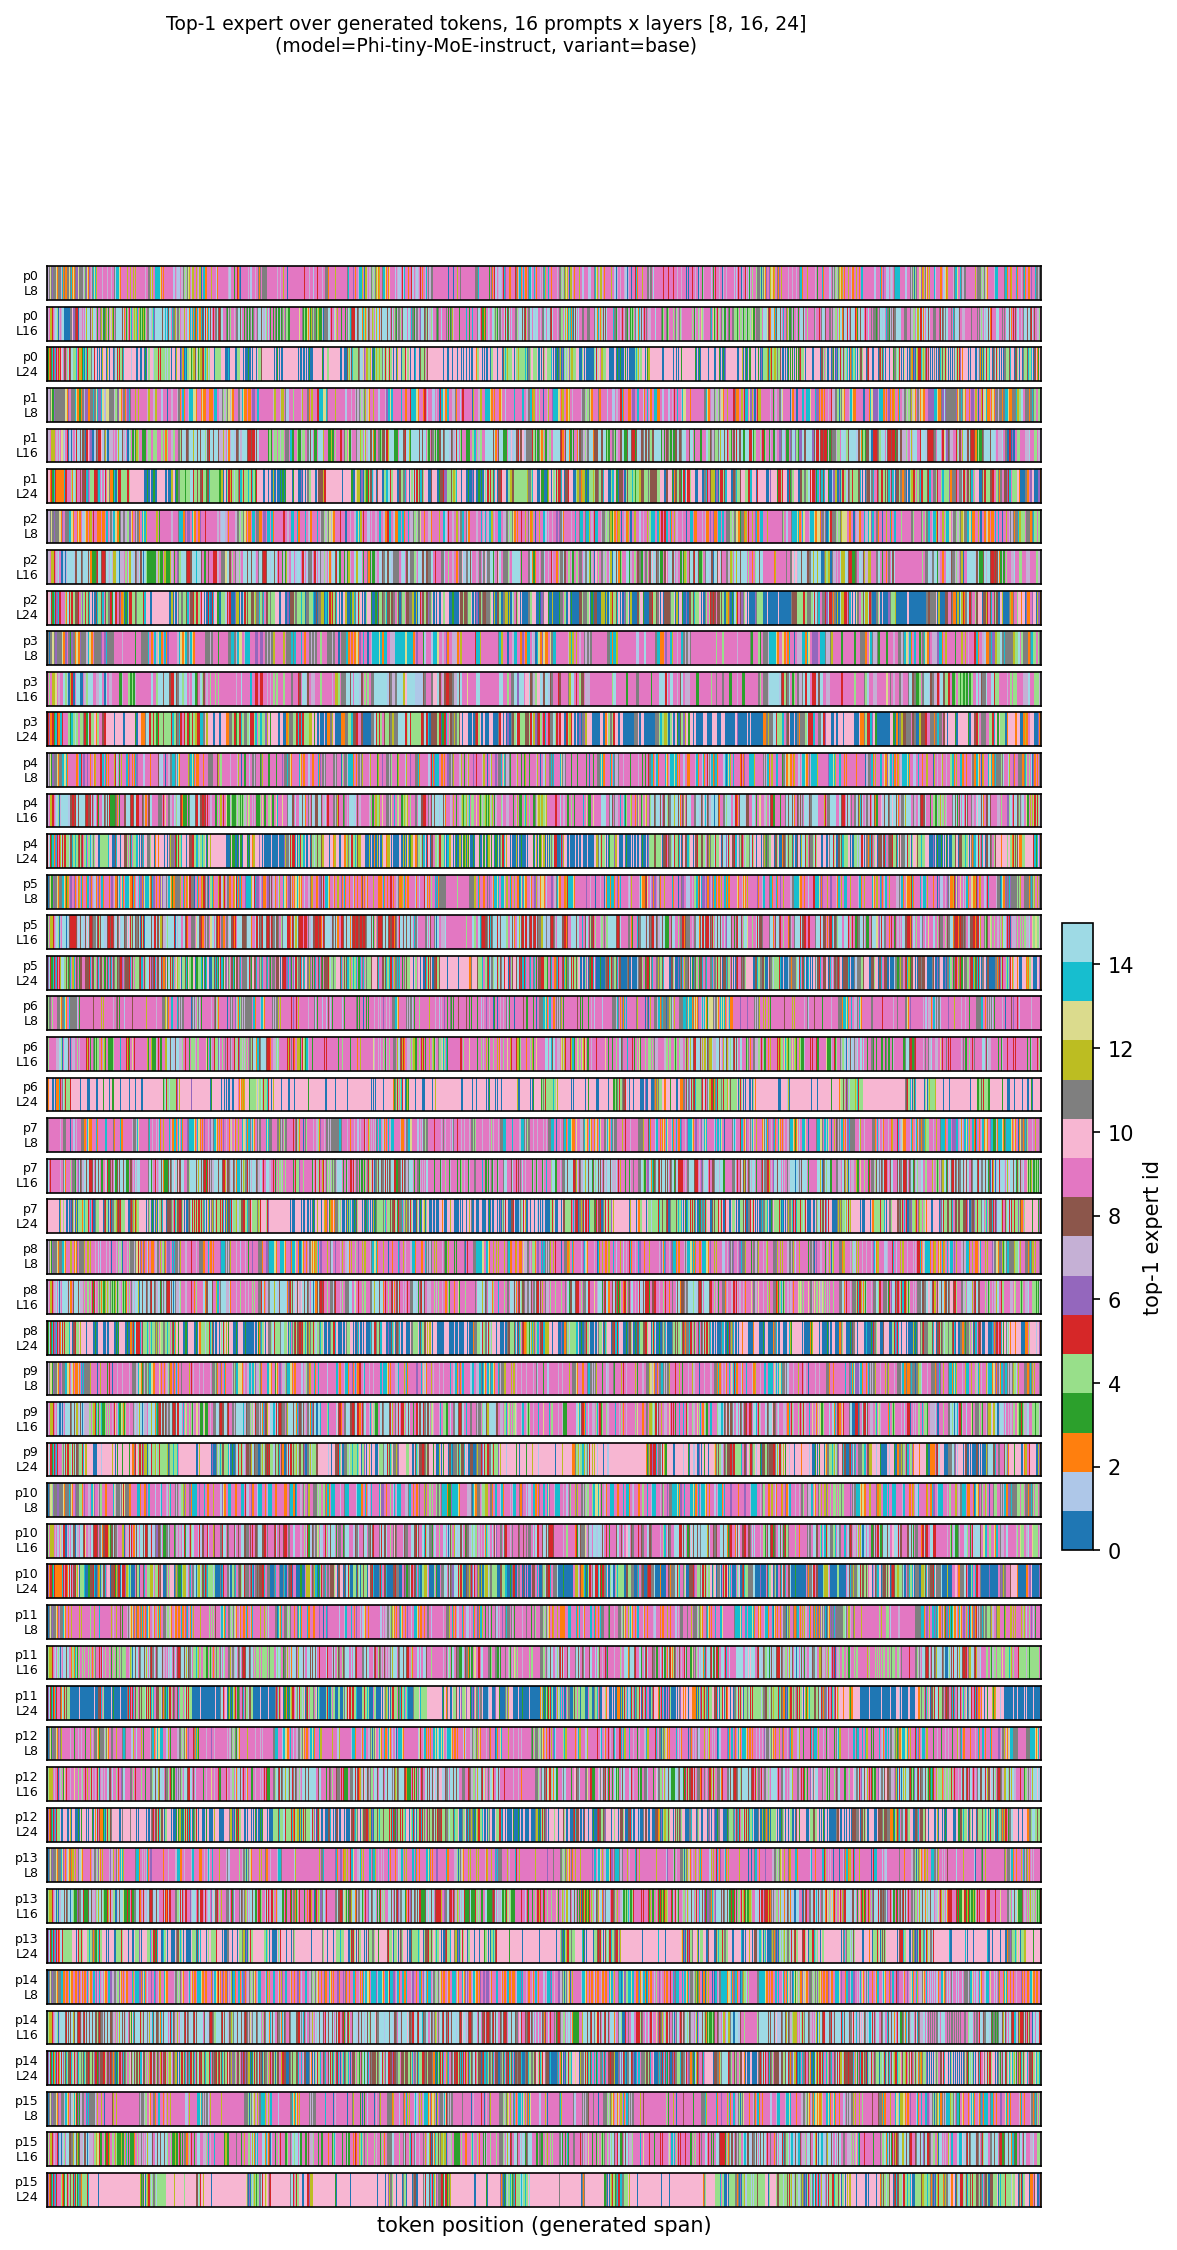
\includegraphics[width=0.55\textwidth]{figures_redundant/phi_base_expert_trace_redundant.png}
\caption{Phi-tiny-MoE-instruct, base (untuned), redundant run.}
\end{figure}

\begin{figure}[h]
\centering
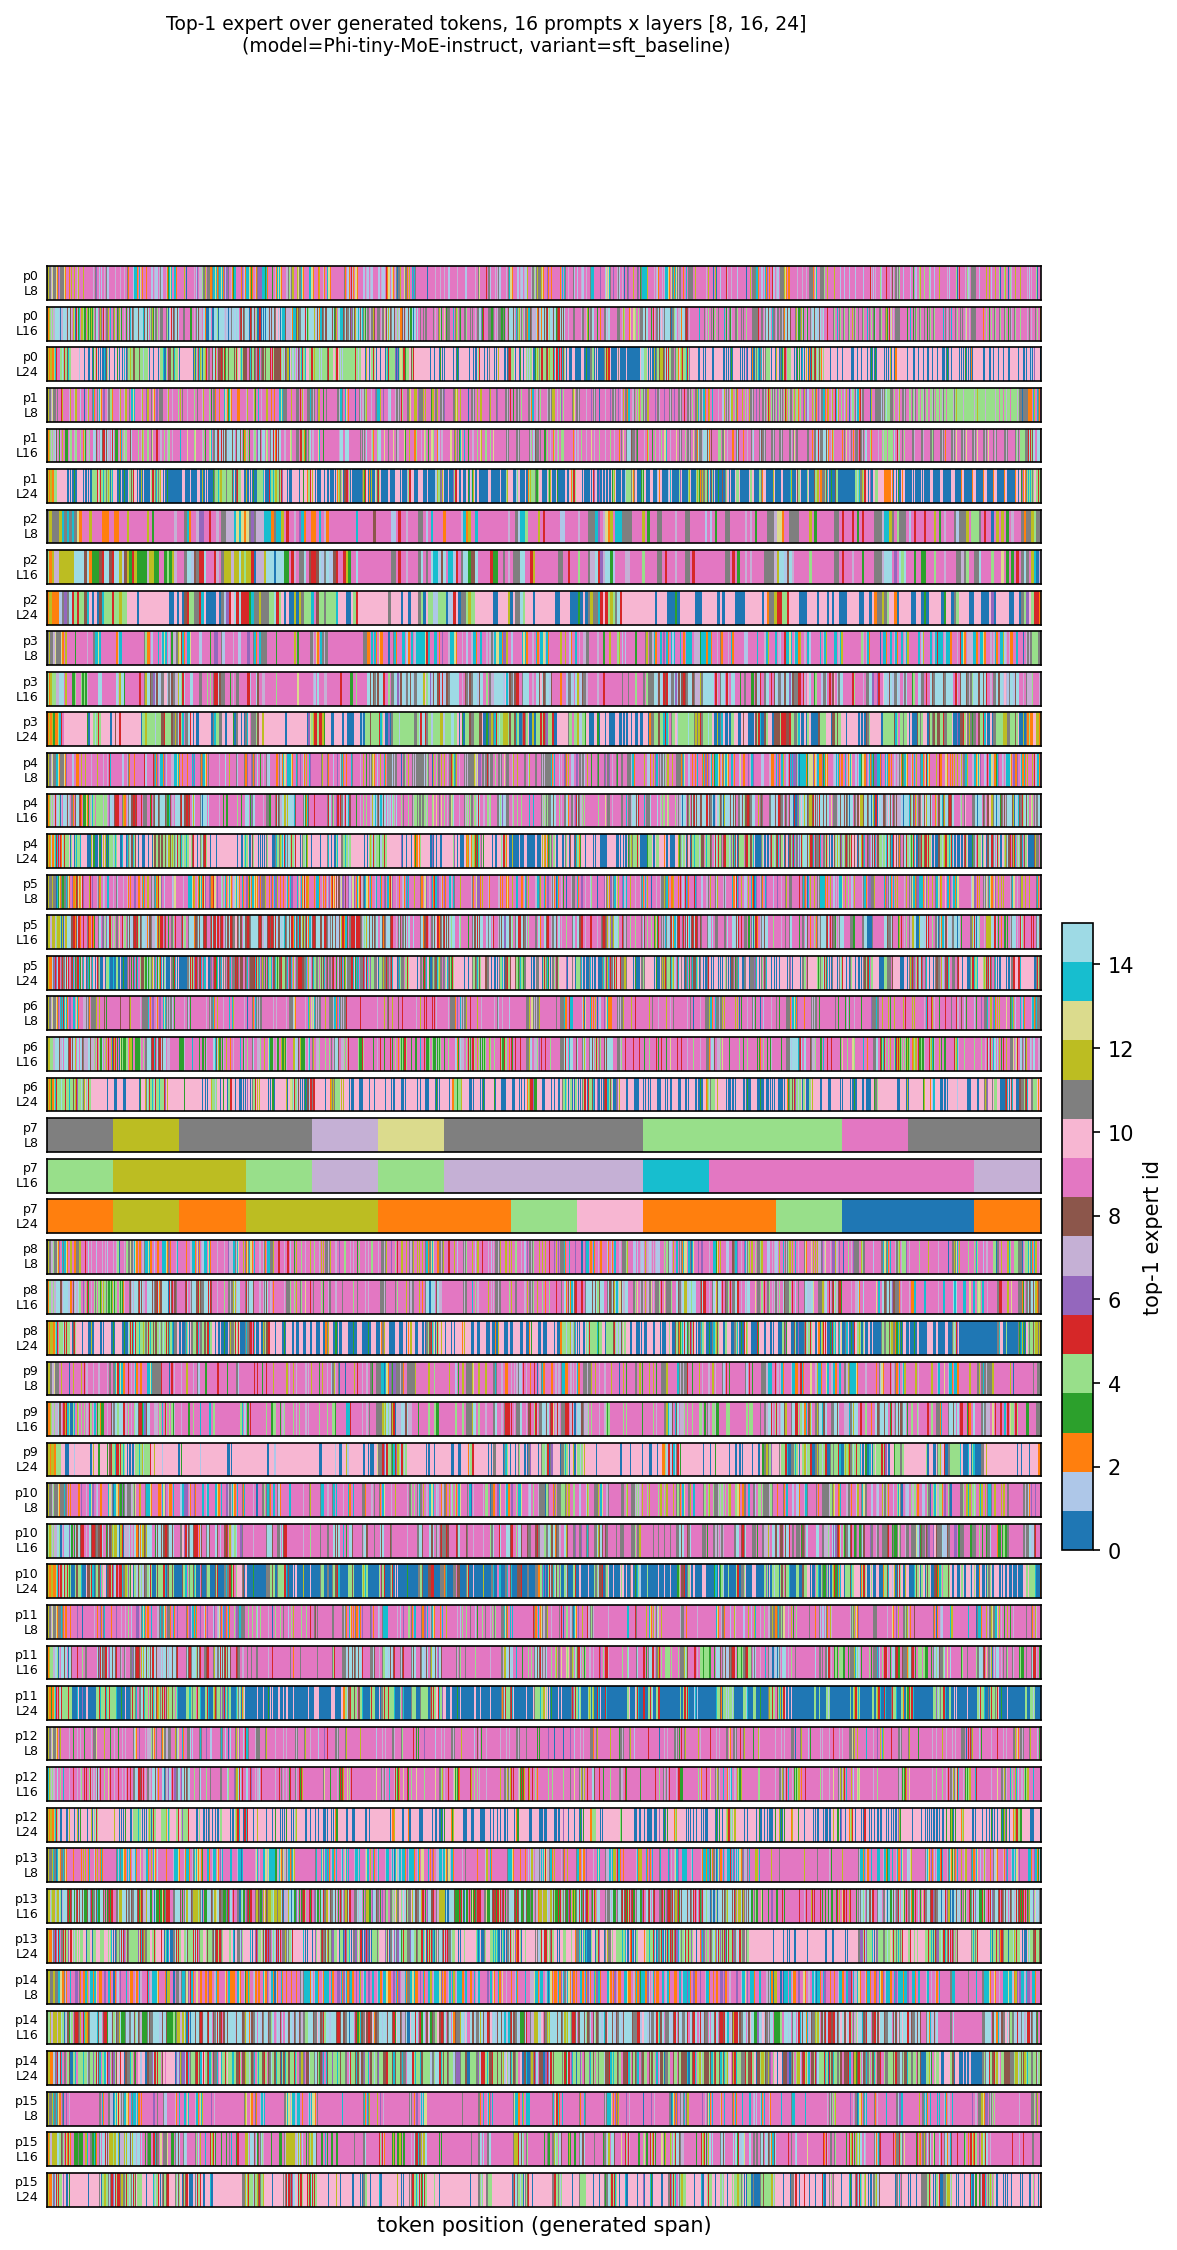
\includegraphics[width=0.55\textwidth]{figures_redundant/phi_sft_baseline_expert_trace_redundant.png}
\caption{Phi-tiny-MoE-instruct, causal LM alone (SFT), redundant run.}
\end{figure}

\begin{figure}[h]
\centering
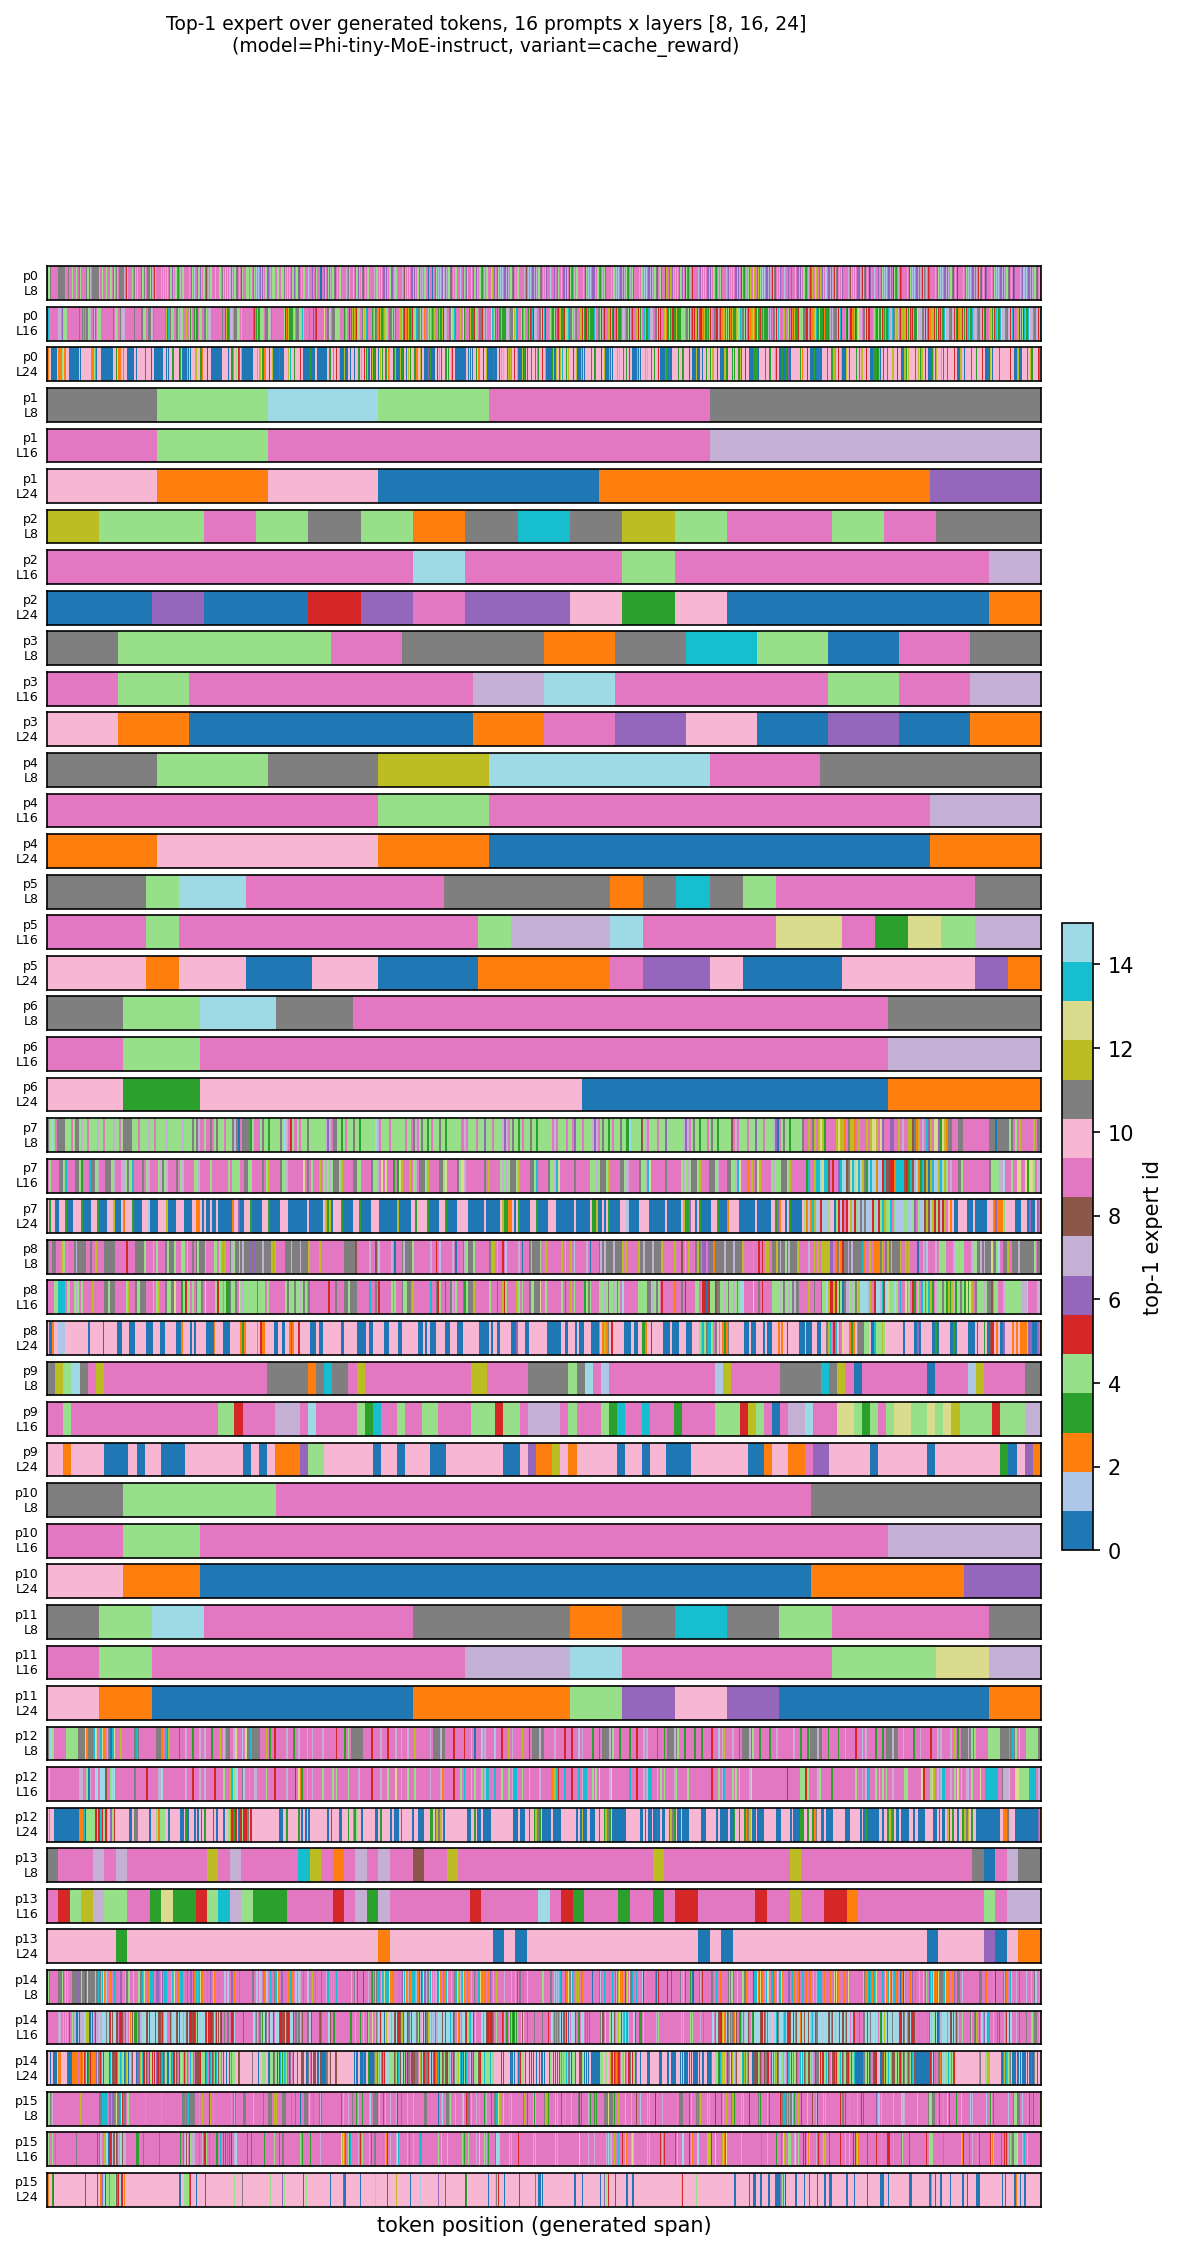
\includegraphics[width=0.55\textwidth]{figures_redundant/phi_cache_reward_expert_trace_redundant.png}
\caption{Phi-tiny-MoE-instruct, working-set reward alone, redundant run.}
\end{figure}

\begin{figure}[h]
\centering
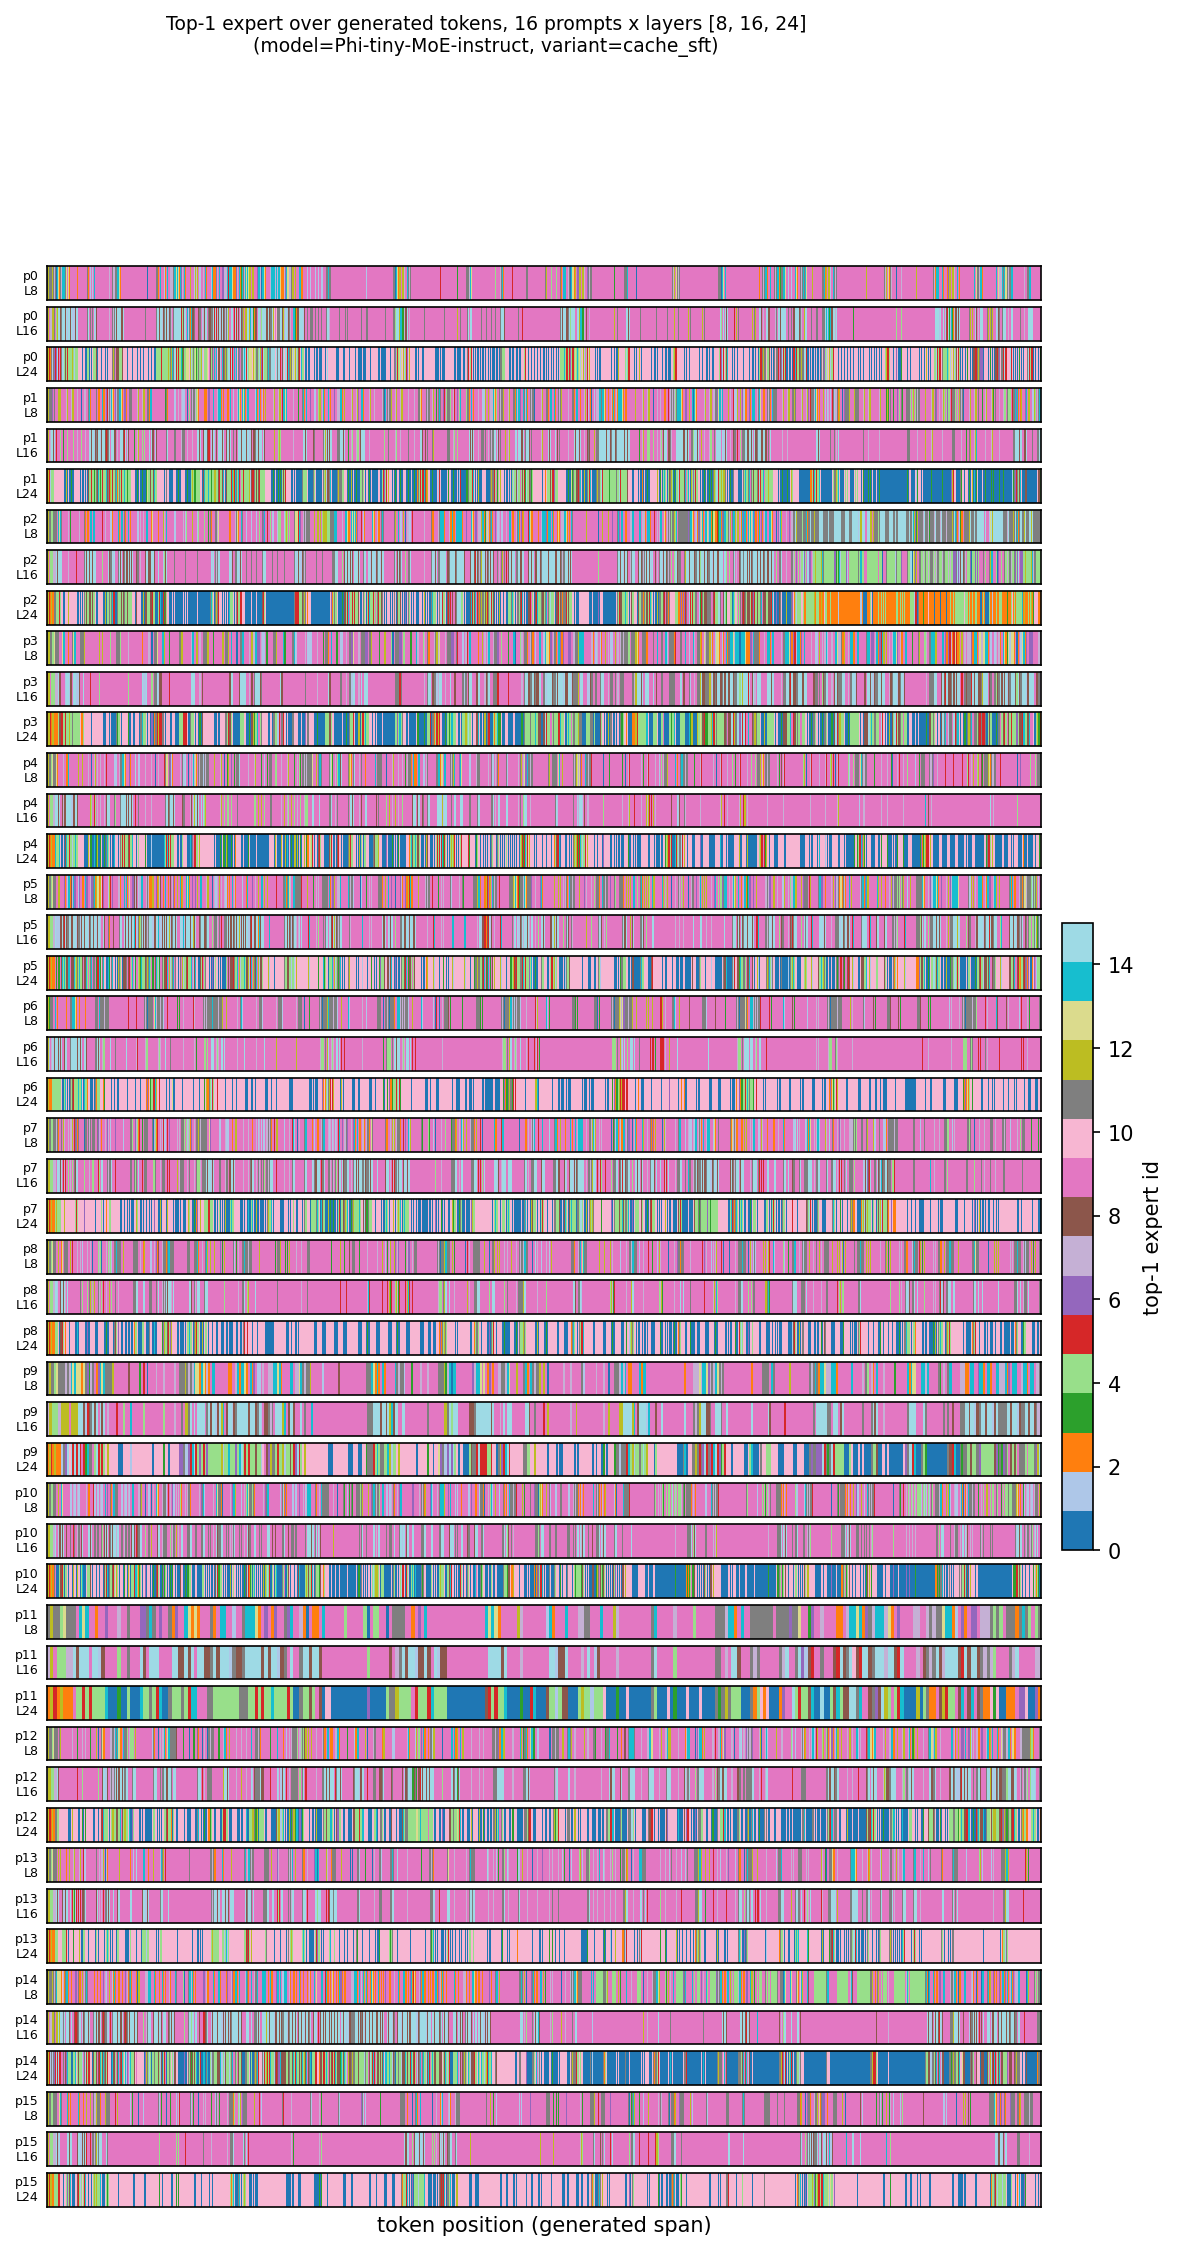
\includegraphics[width=0.55\textwidth]{figures_redundant/phi_cache_sft_expert_trace_redundant.png}
\caption{Phi-tiny-MoE-instruct, working-set reward + SFT, redundant run.}
\end{figure}

\begin{figure}[h]
\centering
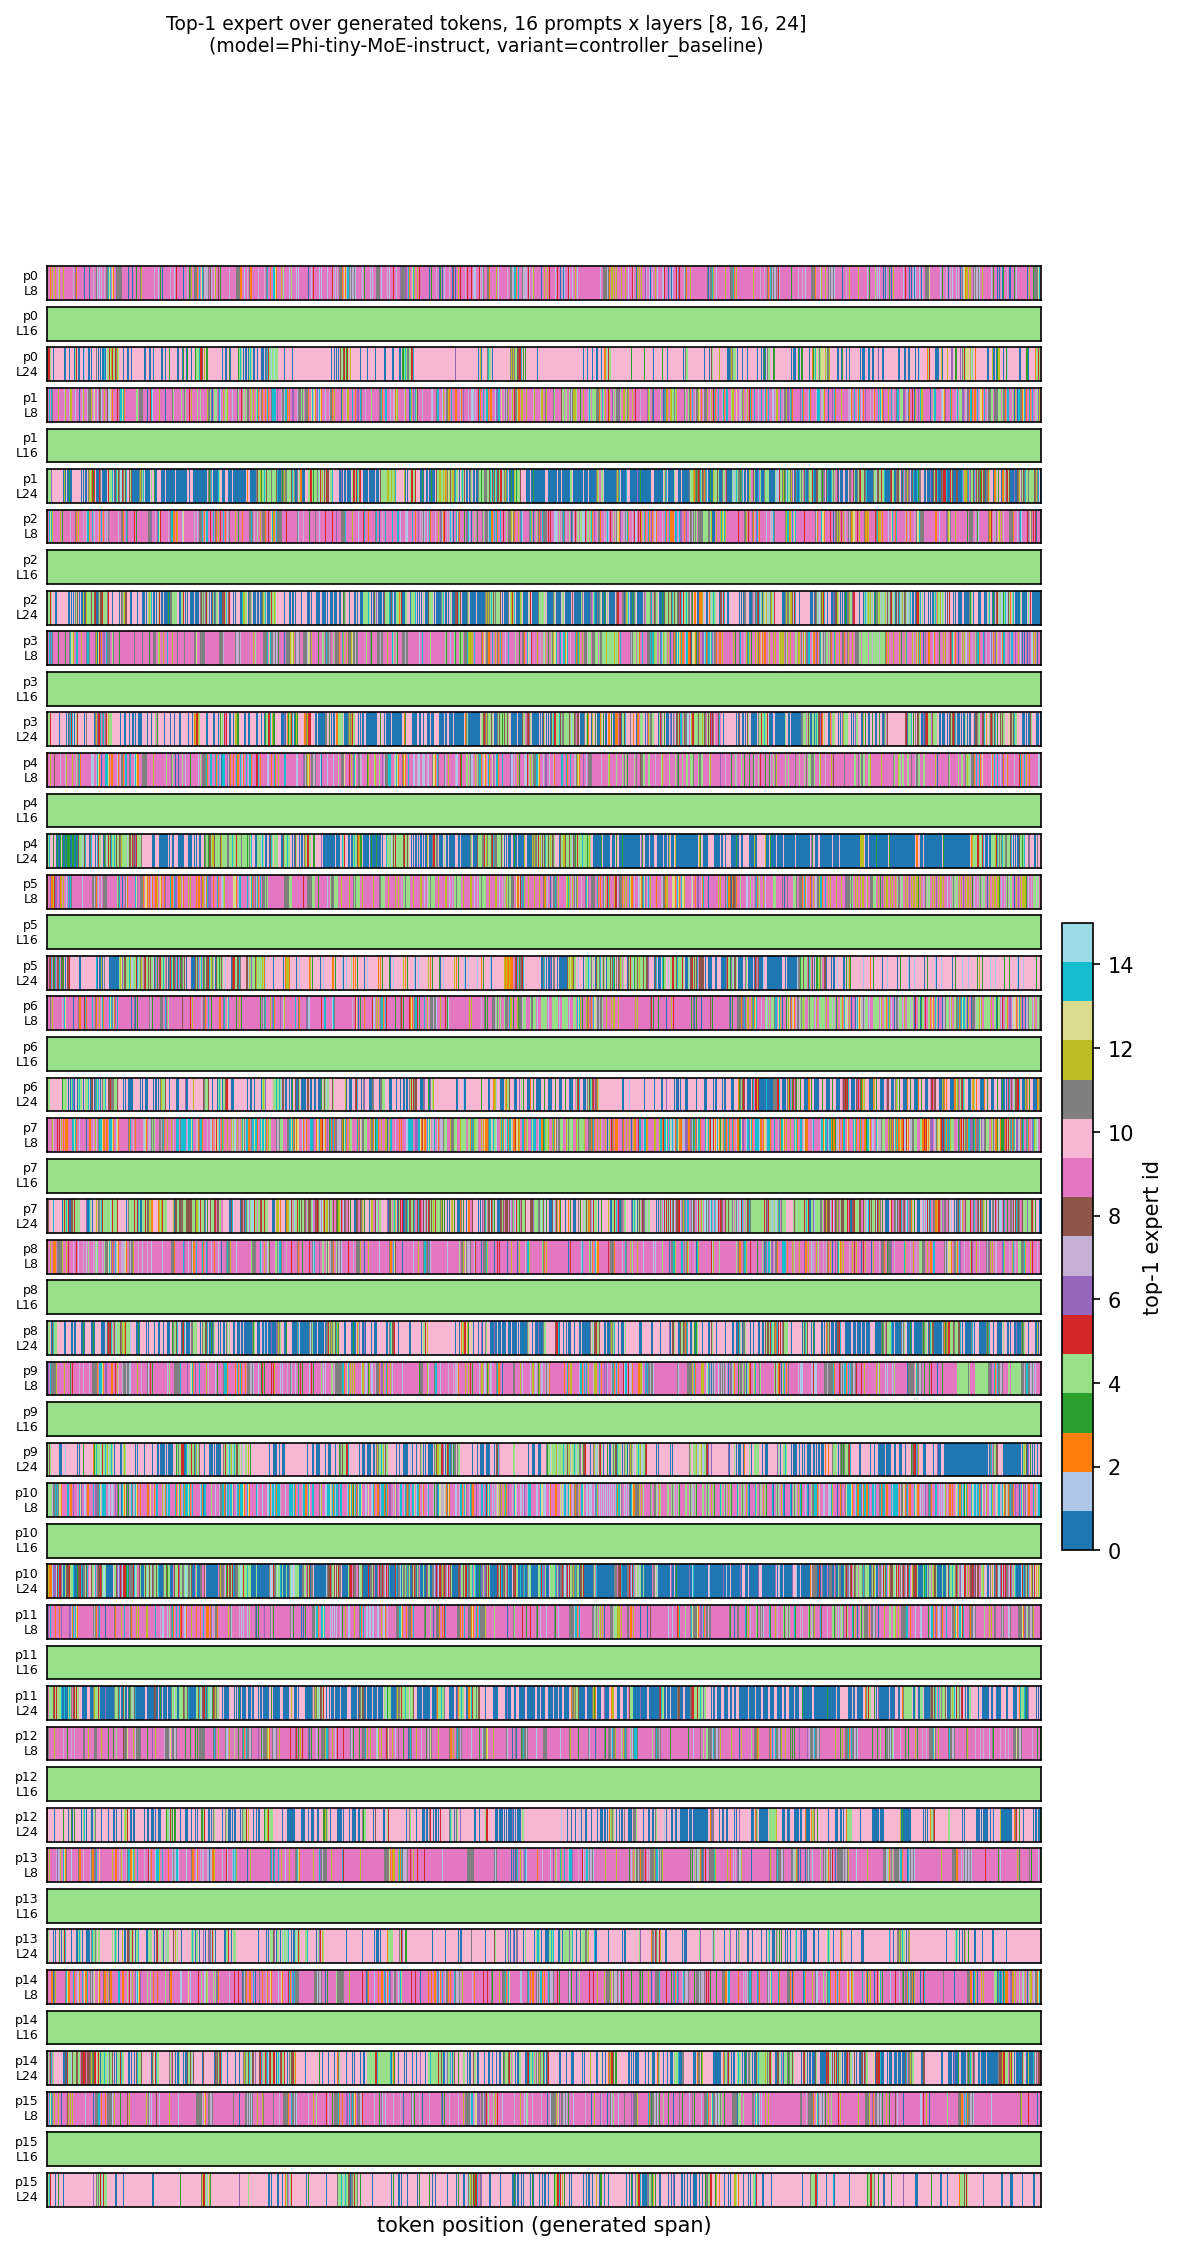
\includegraphics[width=0.55\textwidth]{figures_redundant/phi_controller_baseline_expert_trace_redundant.png}
\caption{Phi-tiny-MoE-instruct, option-critic controller, redundant run.}
\end{figure}

\begin{figure}[h]
\centering
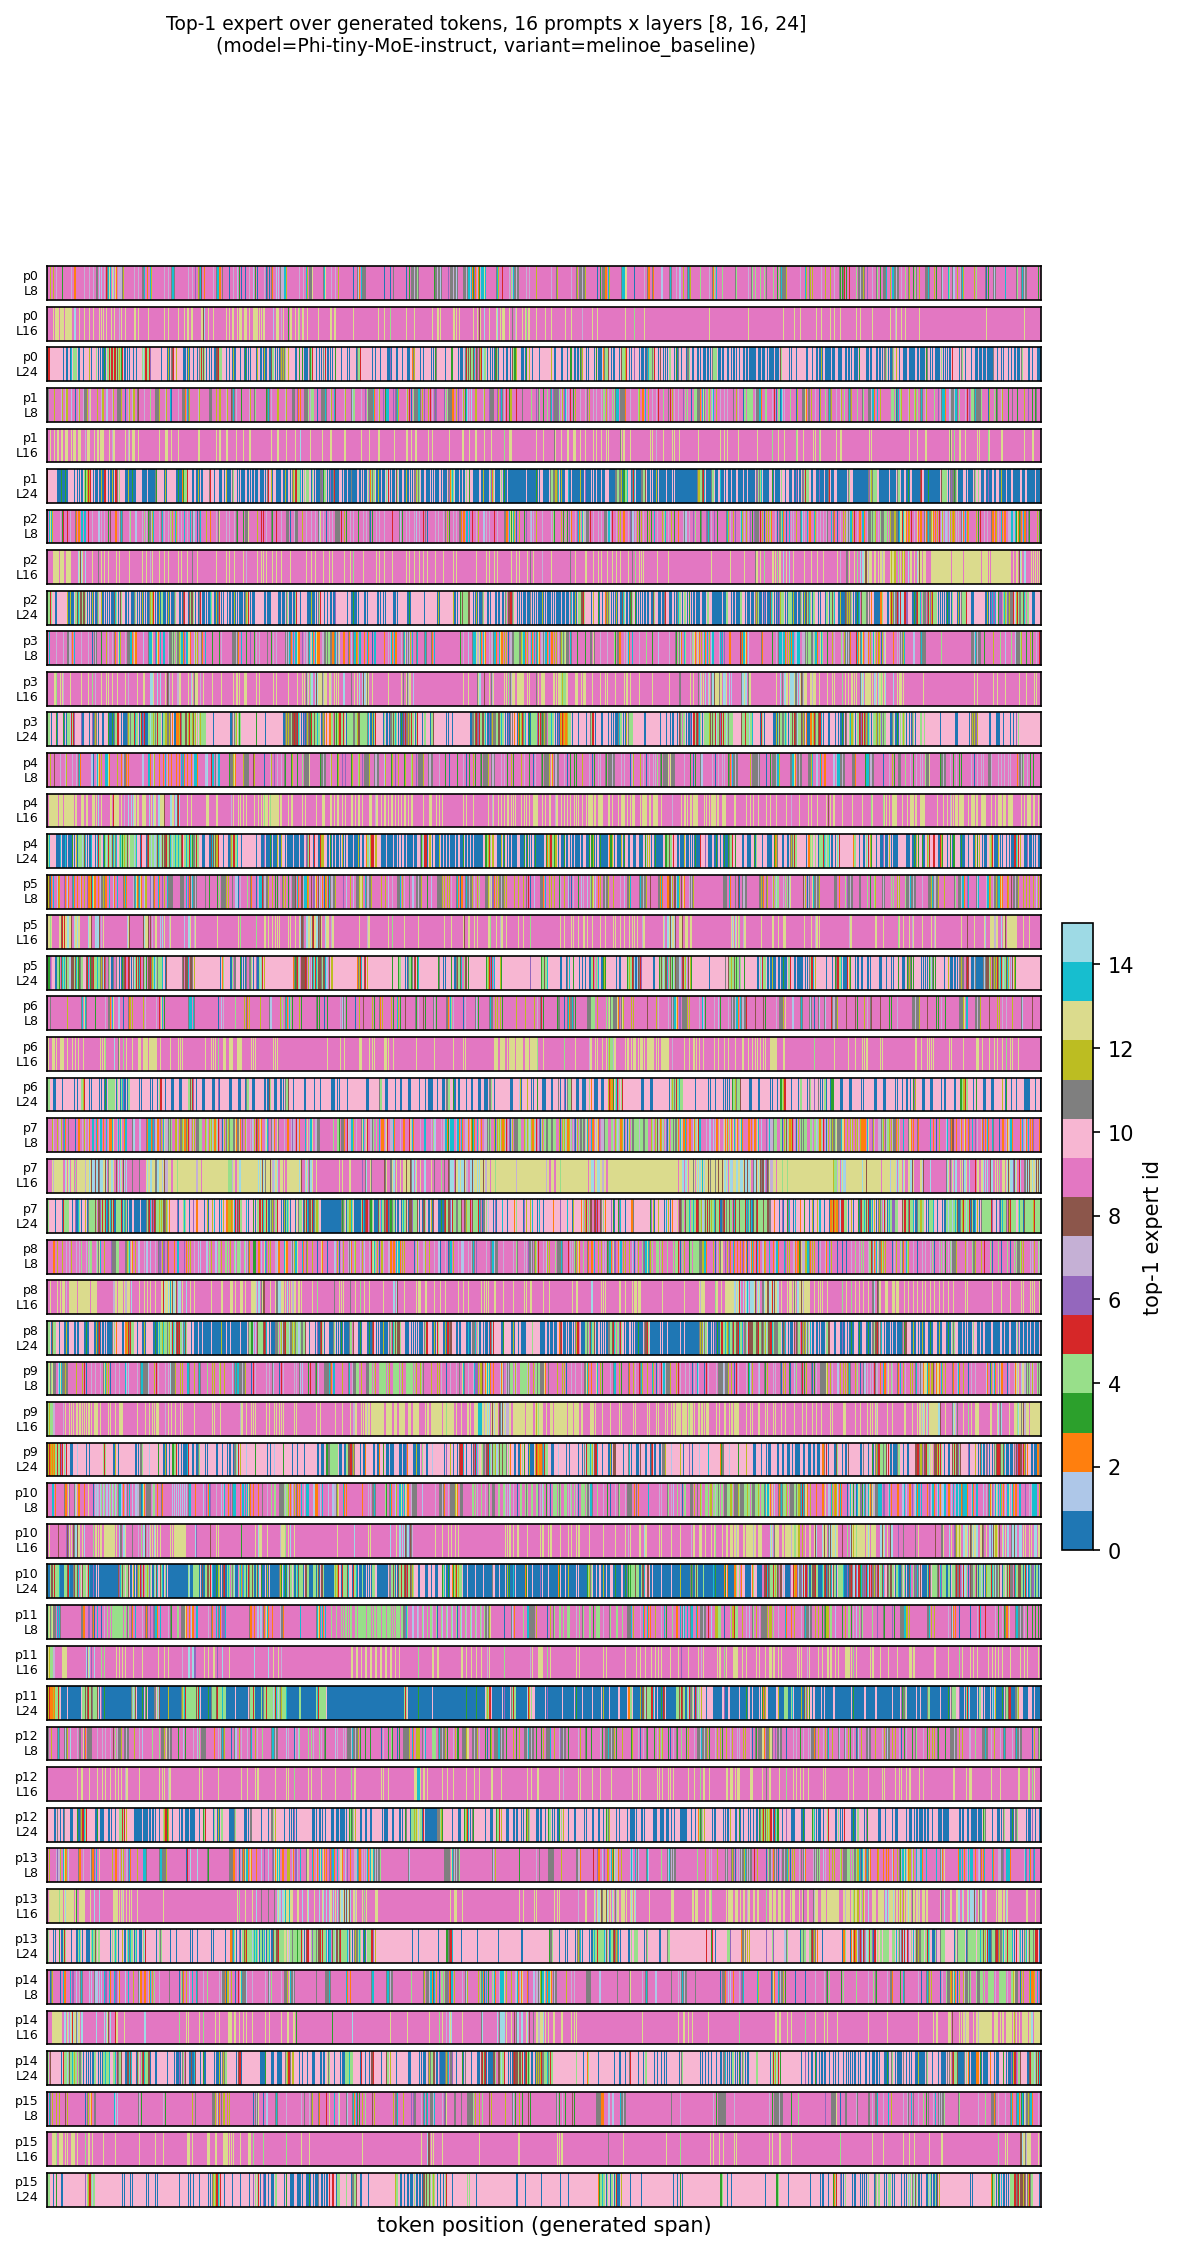
\includegraphics[width=0.55\textwidth]{figures_redundant/phi_melinoe_baseline_expert_trace_redundant.png}
\caption{Phi-tiny-MoE-instruct, MELINOE, redundant run.}
\end{figure}

\begin{figure}[h]
\centering
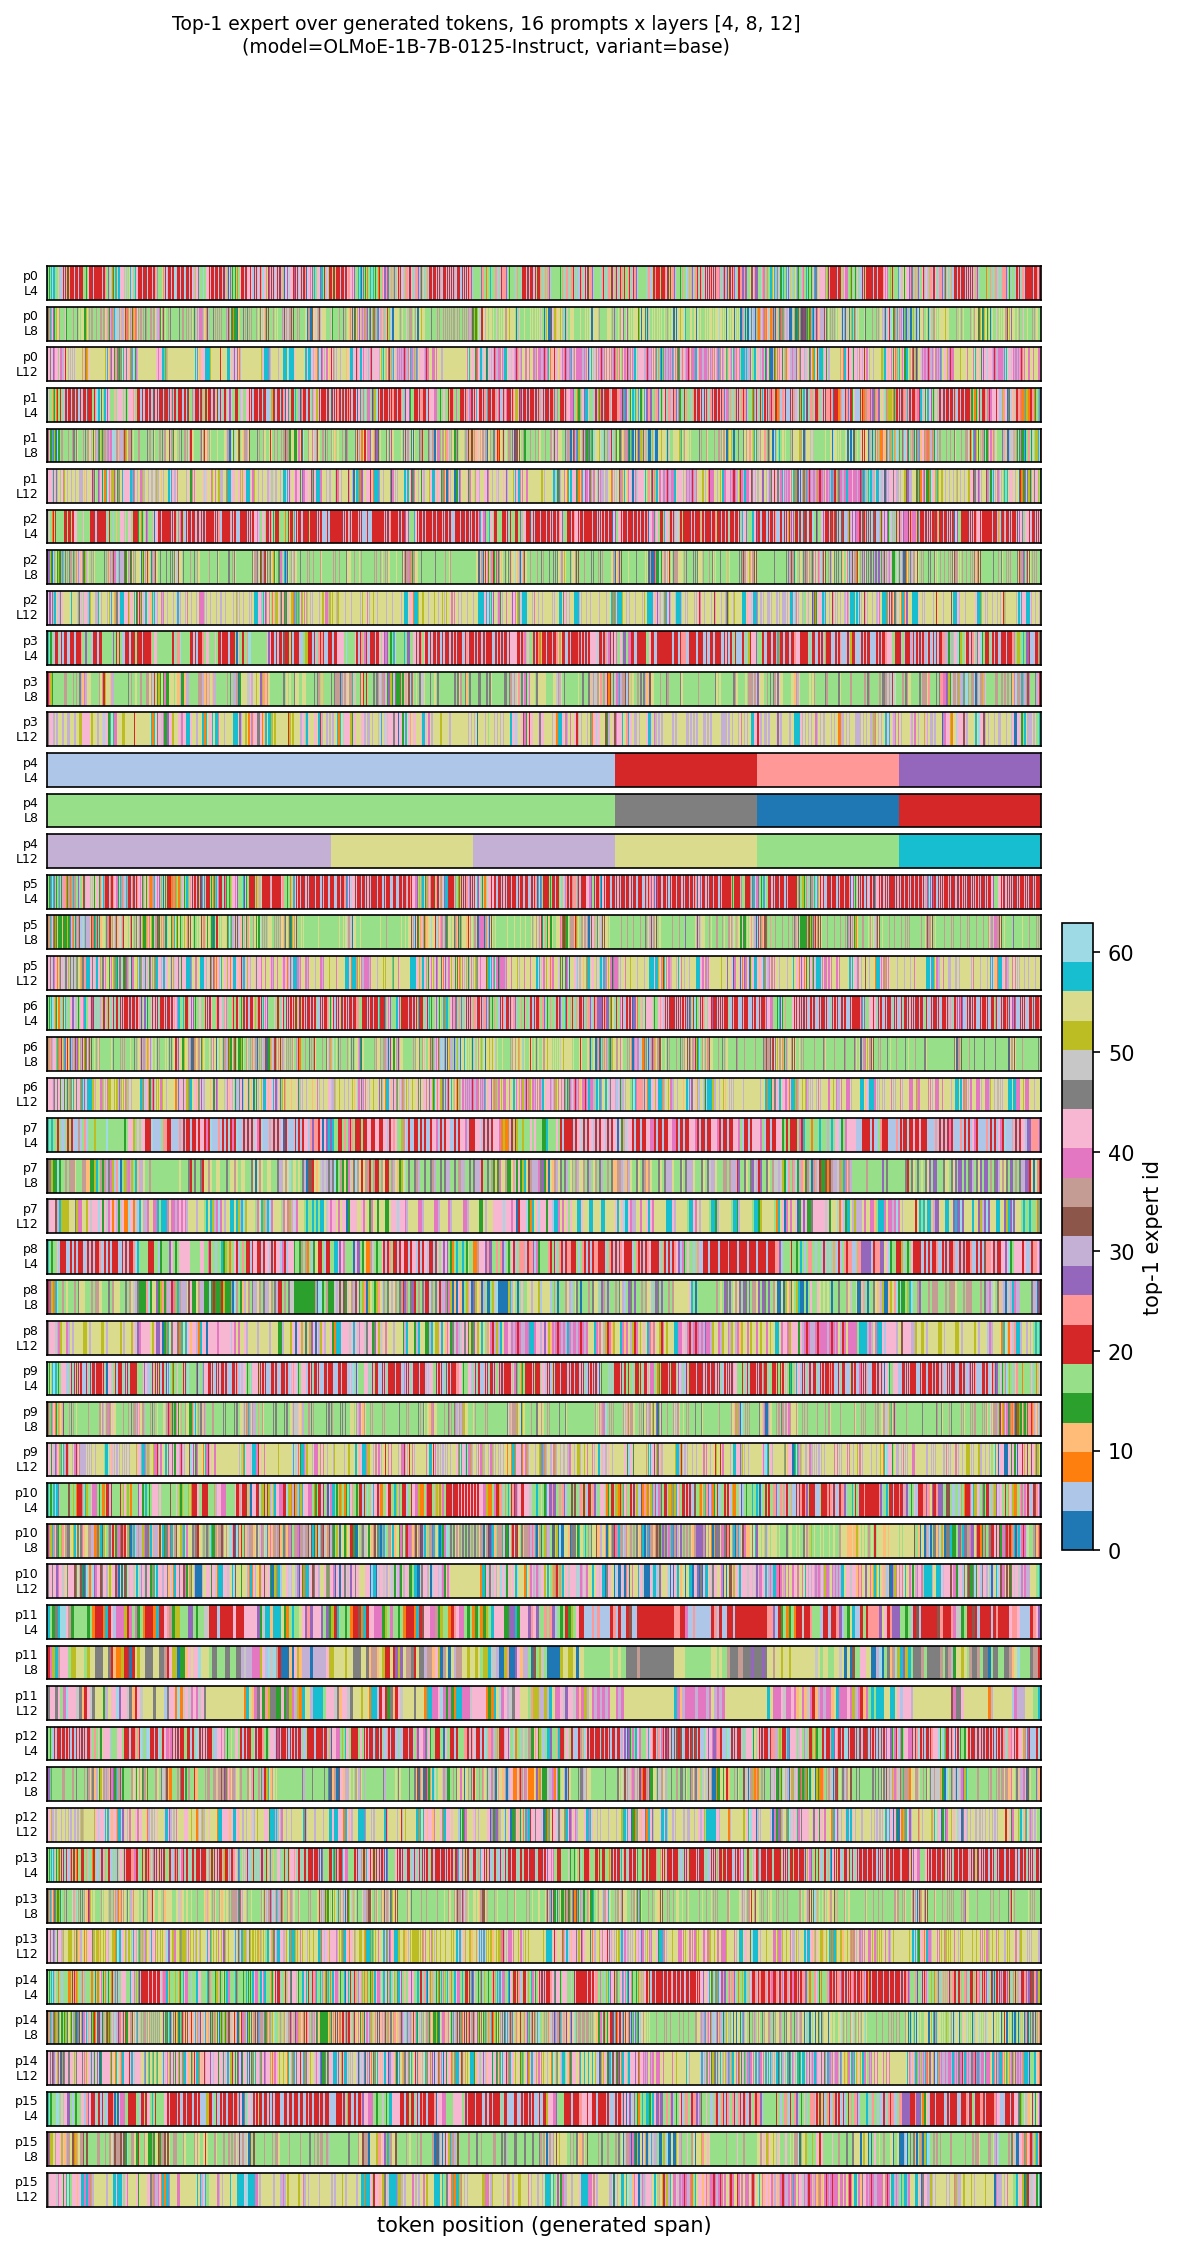
\includegraphics[width=0.55\textwidth]{figures_redundant/olmoe_base_expert_trace_redundant.png}
\caption{OLMoE-1B-7B, base (untuned), redundant run.}
\end{figure}

\begin{figure}[h]
\centering
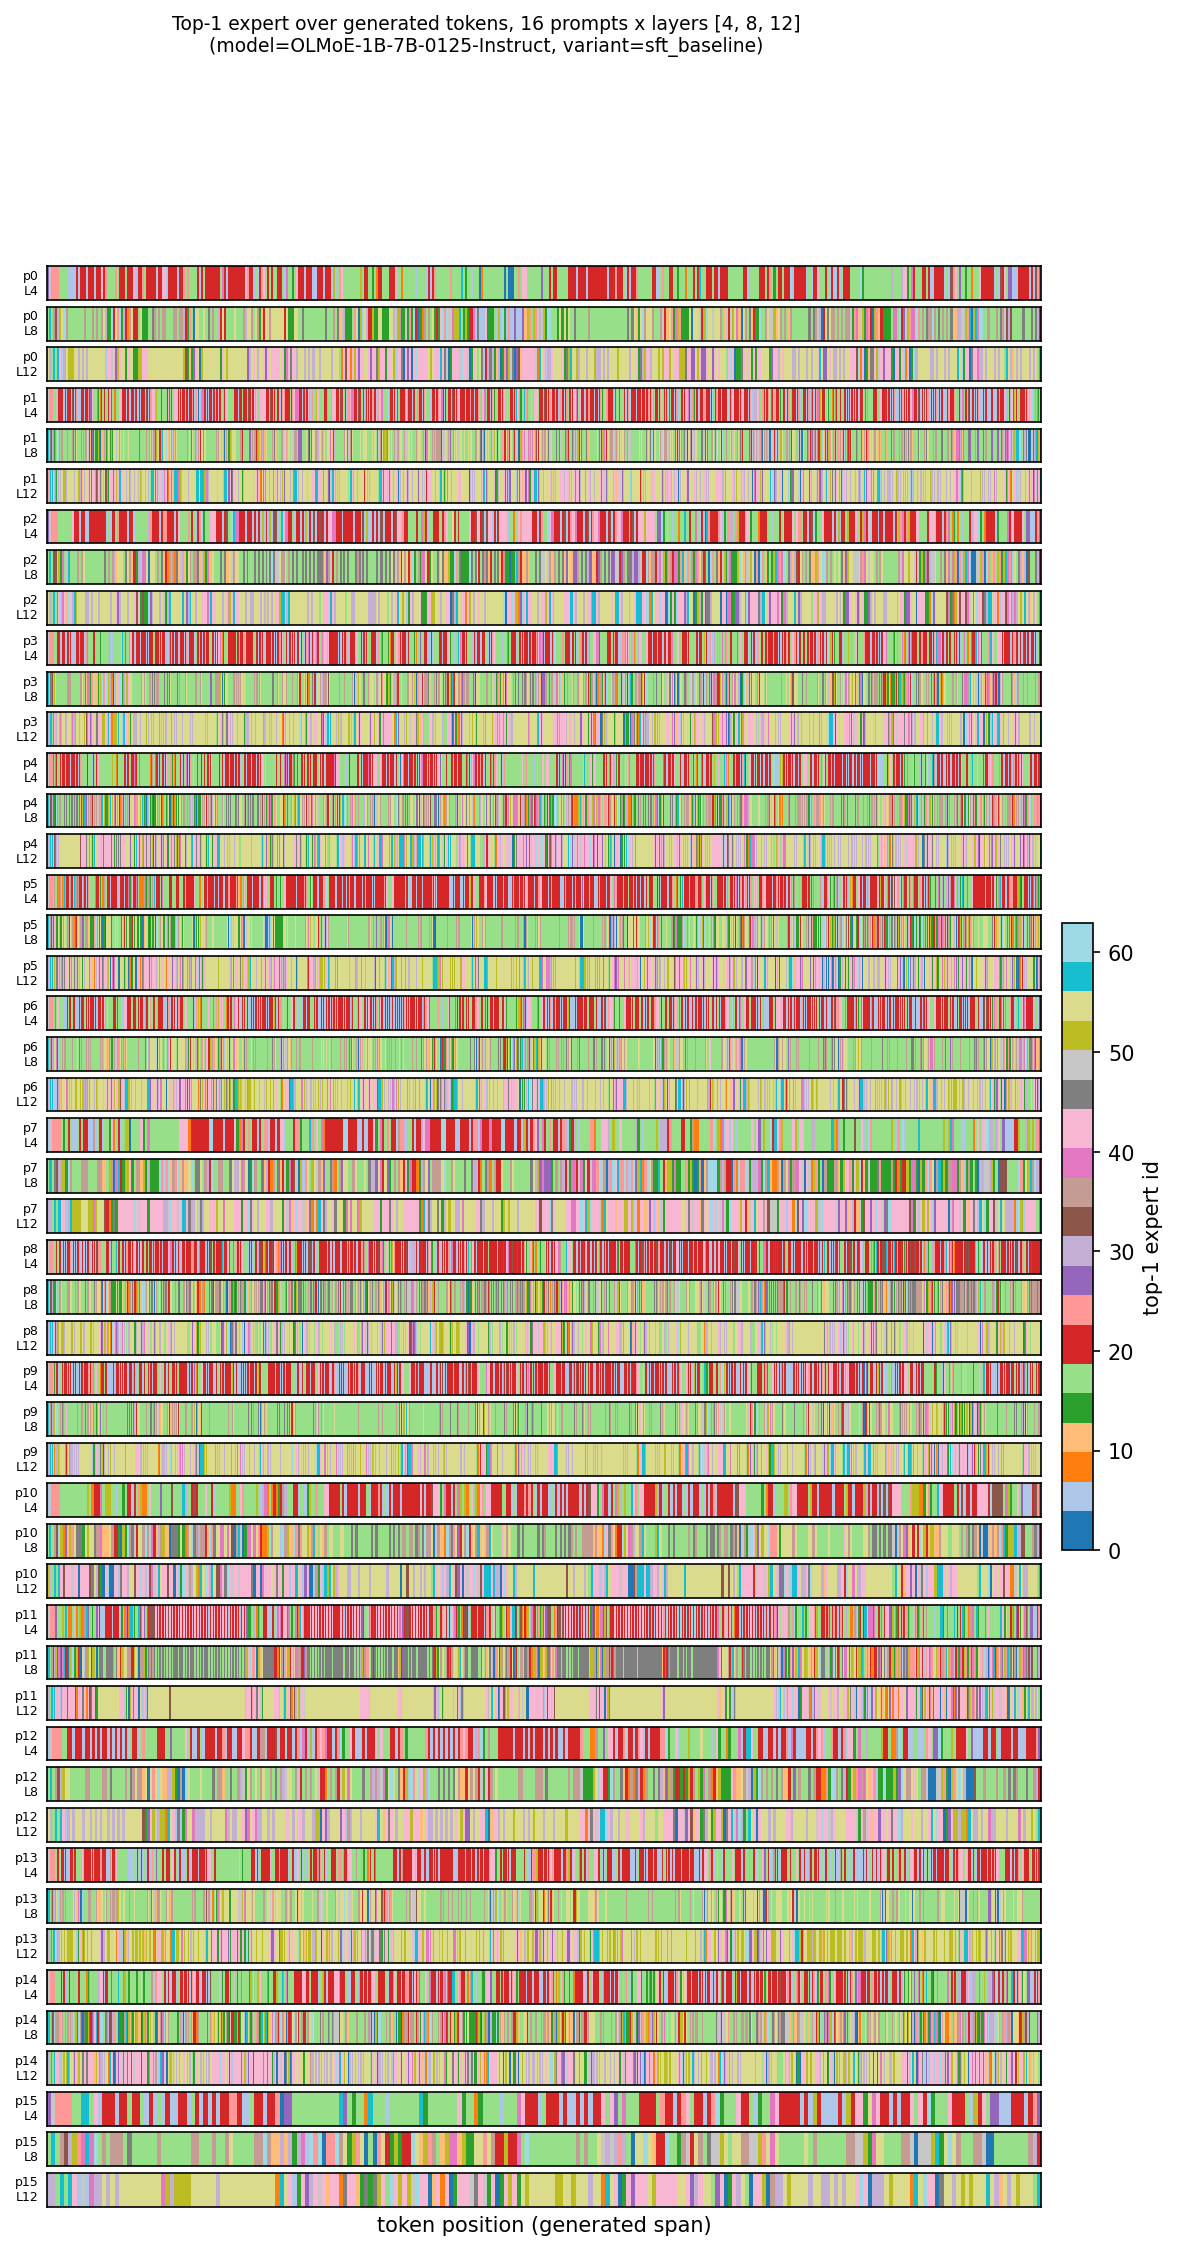
\includegraphics[width=0.55\textwidth]{figures_redundant/olmoe_sft_baseline_expert_trace_redundant.png}
\caption{OLMoE-1B-7B, causal LM alone (SFT), redundant run.}
\end{figure}

\end{document}
